\documentclass[11pt]{beamer}


\usetheme{metropolis}
\usepackage{appendixnumberbeamer}

\usepackage{booktabs}
\usepackage[scale=2]{ccicons}

\usepackage{pgfplots}
\usepgfplotslibrary{dateplot}

\usepackage{fontawesome}

\usepackage{xspace}
\newcommand{\themename}{\textbf{\textsc{metropolis}}\xspace}

\usepackage{outlines}



%---------------------- Math -----------------------------------------------
\usepackage{amsthm}
%\usepackage{amsmath} \newenvironment{smatrix}{\begin{pmatrix}}{\end{pmatrix}} %USUAL
\newenvironment{smatrix}{\left(\begin{smallmatrix}}{\end{smallmatrix}\right)} %SMALL
%\usepackage{nccmath} \newenvironment{smatrix}{\left(\begin{mmatrix}}{\end{mmatrix}\right)} %MEDIUM
\usepackage{amsmath}
\usepackage{amsfonts}

%----------------------Bibliography --------------------------------------
\usepackage[longnamesfirst]{natbib}
\def\citeapos#1{\citeauthor{#1}'s (\citeyear{#1})}
\bibliographystyle{ecta}




%%% Edit graphics path  %%%
\graphicspath{{../../}}

\title{How Emmanuel Macron took over the French electorate}
\subtitle{A Panel analysis using the French National Election Study}
\date{November 29th, 2017}
\author{Marcel Schliebs}
\institute{AM Panel Analysis | Prof. Dr. Michael Scharkow}
\titlegraphic{\hfill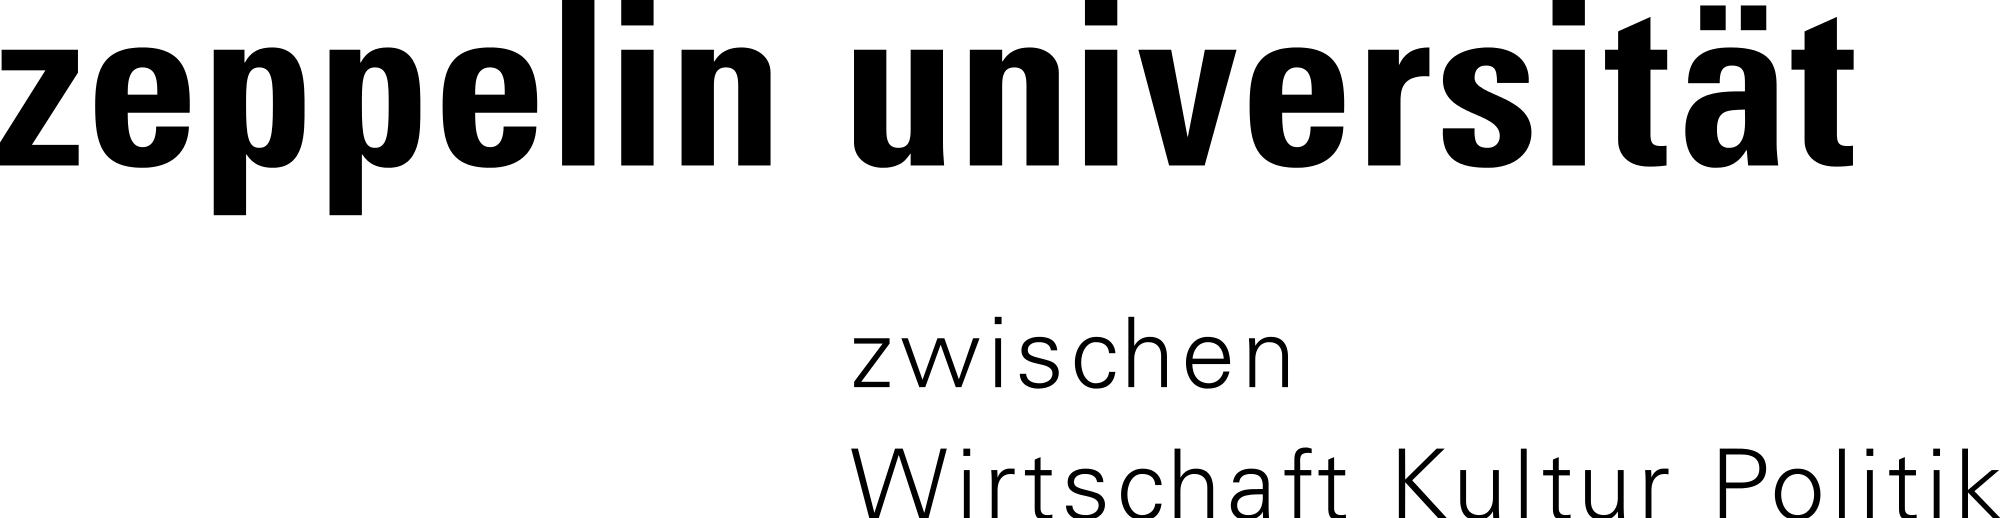
\includegraphics[height=1.0cm]{results/graphics/zu_logo.png}}

\begin{document}

\maketitle

\newpage

\begin{frame}{The French Context - Macron's story}
\begin{enumerate}
	\item unknown within most of electorate + lacking support of major party
	\item rapidly took over french presidential democracy
	\item => securing landslide victory in presidential (66\% in second round) and parliamentary (almost 70\% of seats) elections.
\end{enumerate}
\end{frame}

\begin{frame}{Research Question \& Hypotheses}

\begin{itemize}
	\item<1-|alert@1>{Possible Research questions}
		\only<2-6>{
		\begin{itemize}
			\item<2-6 |alert@2> Were personal candidate considerations or policy orientations decisive?
			\item<3-6 |alert@3> Which were decisive policies with which he convinced voters? 
			\item<4-6 |alert@4> What role did tactical/strategic incentives play?
			\item<5-6 |alert@5> Voters from which ideological positions did EM attract?
			\item<6-6 |alert@6> Did voters with larger ideological gaps to EM switch for him later in the campaign?
		\end{itemize}
		}
	\item<7-|alert@7>{Hypotheses}
			\only<8->{
		\begin{itemize}
			\item<8- |alert@8> H1: A greater ideological distance to EM and his platform leads to a smaller probability of voting for him. (\textit{Downs'ian Rational Voter})
			\item<9- |alert@9> H2: The larger the ideological distance to Macron, the later the switching happend, as polls indicated that there was no reasonable alternative to EM (\textit{Strategic Voting consideration})

		\end{itemize}
	}
\end{itemize}
\end{frame} 

\begin{frame}{Data}

\begin{itemize}
	\item<1-|alert@1>{CEVIPOF-ENEF (\textit{Enquete Electorale Francaise})}
	\only<2-6>{
		\begin{itemize}
			\item<2-6 |alert@2> Longitudinal Panel
			\item<3-6 |alert@3> 16 waves from Nov 2015 to Jul 2017
			\item<4-6 |alert@4> 25000 original observations, thereof 15000 who completed all questionnaires (=> low mortality)
			\item<5-6 |alert@5> Effective Survey weights => Using them, I was able to forecast the first round with less than 0.5 percentage points on average for each of the 6 main candidates
			\item<6-6 |alert@6> thousands of variables, also experiments implemented
		\end{itemize}
	}
	\item<7-|alert@7>{Variables \& Operationalization}
	\only<8->{
		\begin{itemize}
			\item<8- |alert@8> Dep.Var: \textit{Vote for Emmanuel Macron (0|1)}
			\item<9- |alert@9> Ind.Var I: \textit{Ideological Distance to En Marche}
			\item<10- |alert@10> Ind.Var II: \textit{Wave: (measured in months until election?)}
			\item<11- |alert@11> Other Covariates: \textit{the usual Michigan-model control variables}
		\end{itemize}}
\end{itemize}
\end{frame} 

\begin{frame}{Model building}

\begin{itemize}
	\item<1-|alert@1>{Model propositions (\textit{Need some more dirty data cleaning before I start analysis})}
	\only<2-4>{
		\begin{itemize}
			\item<2-4 |alert@2> Base-Mod I:\\ $glmer(macron \sim wave + (1 | id), data, family = binomial())$ [\textit{random intercept for ids}]
			\item<3-4 |alert@3> Mod II:\\ $glmer(macron \sim wave * ideol\_distance + (1 + wave | id), data, family = binomial())$ [\textit{additional random slope for wave}]
			\item<4-4 |alert@4> Mod III?: further include $wave:ideol\_distance|id)$ [\textit{including random intercept and slope for interaction effect}]
		\end{itemize}
	}
	\item<5-|alert@5>{Outlook: Bayesian Model}
	\only<6-7>{
		\begin{itemize}
			\item<6-7 |alert@5> Powerful model for estimating many random effects
			\item<7-8 |alert@6> Implementation in STAN
	\end{itemize}}
\end{itemize}
\end{frame} 



%
\begin{frame}{Discussion \& Feedback}
Thank you for you kind attention!\\
presentation, code,  \only<2-4>{\textbf{but no data yet(sorry!)}}\\
on \faGithub  \href{github.com/schliebs/enef\_panel}{github.com/schliebs/enef\_panel}\\
\only<3-3> {Zum Abschluss noch 1 Meme}
\only<4-4> {Zum Abschluss noch 2 Memes}

\begin{figure}[ht!]
	\begin{center}
		%
		\only<3-4> {\subfigure{%
				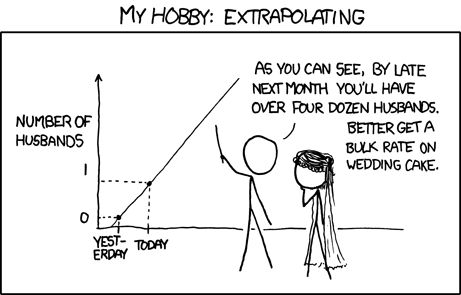
\includegraphics[width=0.4\textwidth]{results/images/weddingcake_jpg.jpg}
			}%
		}
		\only<4-4>{
			\subfigure{%
				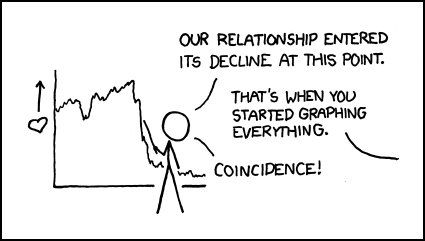
\includegraphics[width=0.4\textwidth]{results/images/coincidence_jpg.jpg}
			}
		}
		
	\end{center}
\end{figure}5\end{frame}


\end{document}
